\chapter{Additional content}


\section{Unity Robotics Hub Overview}

    Before diving into the specifics of establishing the ROS-Unity connection and further develop the project, both tutorials and resources available 
    in the Unity Robotics Hub were studied. This GitHub repository serves as a central hub for tools, tutorials, and documentation tailored for robotic 
    simulation in Unity.

    \subsection{Available Documentation}

    It offers a range of tutorials that are invaluable for setting up and extending ROS-Unity integration, as well as to understand how ROS concepts work inside Unity's environment:
    
    \begin{itemize}
        \item \textbf{ROS–Unity Integration: Initial Setup} - Guides you through the initial steps of setting up communication between ROS and Unity, including package installation and network configuration.
        
        \item \textbf{ROS–Unity Integration: Network Description} - Provides a detailed overview of network settings and offers troubleshooting tips for connectivity issues.
        
        \item \textbf{ROS–Unity Integration: Publisher} - Teaches you how to publish messages from a Unity scene to ROS, with practical examples involving GameObject data.
        
        \item \textbf{ROS–Unity Integration: Subscriber} - Demonstrates how to subscribe to ROS topics in Unity and use the received messages to alter objects in a Unity scene.
        
        \item \textbf{ROS–Unity Integration: Unity Service} - Covers the implementation of ROS services within Unity, allowing Unity to respond to ROS service requests.
        
        \item \textbf{ROS–Unity Integration: Service Call} - Explains how to call external ROS services from Unity, enabling Unity to request data or actions from ROS nodes.
    \end{itemize}
    
    The repository also includes example scripts that correspond to each tutorial.
    
    \section{Establishing the Network Connection}
    After reviewing the Unity Robotics Hub tutorial on network integration, it became clear that establishing a network connection between the Unity and ROS environments was the first crucial step in remote application development. The process involves:
    \begin{itemize}
        \item \textbf{Setting up the network:} Connect the Unity laptop to a Wi-Fi network, then connect the Ubuntu laptop running ROS to the hotspot created by the Unity laptop.
        \item \textbf{Configuring the IP address:} Use the IP address from the Unity laptop within the Unity inspector as shown in Figure \ref{fig:unity_connection}, and in the \texttt{ROSConnection.cs} script to ensure proper communication.
        \item \textbf{Specify the IP Address in ROS Workspace:} A new \textit{.launch} file was created to initialize new nodes, including the \texttt{server\_endpoint} node from the \texttt{ros\_tcp\_endpoint} package, crucial for establishing a proper connection between the ROS and Unity environments. An example of the IP definition in the \textit{.launch} file can be seen below.
    \end{itemize}
    
    \begin{figure}[htbp]
        \centering
        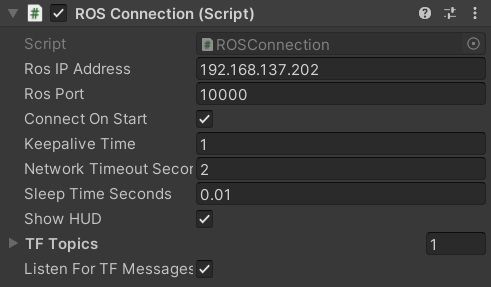
\includegraphics[width=0.5\linewidth]{figs/connection_inspector.png}
        \caption{Unity Connection Inspector}
        \label{fig:unity_connection}
    \end{figure}
    
    % \begin{figure}[htbp]
    %     \centering
    %     \includegraphics[width=\linewidth]{tcp_ip_connection_launch.jpg}
    %     \caption{TCP/IP ROS Node Connection Setup}
    %     \label{fig:tcp_ip_connection}
    % \end{figure}
    \begin{verbatim}
            <arg name="tcp_ip" default="192.168.137.202"/>
            <arg name="tcp_port" default="10000"/>
            
            <node name="server_endpoint" pkg="ros_tcp_endpoint" 
                type="default_server_endpoint.py" args="--wait" output="screen" 
                respawn="true">
                <param name="tcp_ip" type="string" value="$(arg tcp_ip)"/>
                <param name="tcp_port" type="int" value="$(arg tcp_port)"/>
            </node>
    \end{verbatim}
    
    
    This setup is fundamental for the Unity environment to interact effectively with ROS, allowing for real-time data exchange and control commands to be sent between the two systems. Further details are available in the Unity Robotics Hub tutorial on \href{https://github.com/Unity-Technologies/Unity-Robotics-Hub/blob/main/tutorials/ros_unity_integration/network.md}{ROS-Unity integration}.


    \section{ROS Message Generation}
    
    After establishing the communication between ROS and Unity, as well as the other basic communication channels—publishers, subscribers, and services, the next step was to customize these components to handle the specific types of messages required for this project.
    
    \subsection{Adapting to Specific Message Types}
    
    To begin, I revisited the previously mentioned GitHub repositories for the UR10e robot, specifically focusing on identifying which ROS nodes and topics were critical for my Unity-ROS integration. This involved:
    \begin{itemize}
        \item \textbf{Identifying Key Nodes and Topics:} The primary focus was on 
        % the \texttt{/joint\_states} topic,
        finding which topic is responsible for publishing the current state of the robot’s joints.
        \item \textbf{Message Subscription and Retrieval:} With guidance from my supervisors, I determined that subscribing to the \texttt{/joint\_states} topic would be essential for retrieving real-time data about the robot's joint positions.  This topic uses the \texttt{sensor\_msgs/JointState} message type, a standard message in ROS that provides the positions, velocities, and efforts of the robot's joints. It is well-documented and includes the necessary fields for capturing joint states. This message type is part of the broader \texttt{common\_msgs/sensor\_msgs} package, which is available on the \href{https://wiki.ros.org/sensor_msgs}{ROS wiki} and in the \href{https://github.com/ros/common_msgs/tree/noetic-devel/sensor_msgs/msg}{sensor\_msgs GitHub repository}.
    \end{itemize}
    
    \subsection{ROS-TCP Connector and C\# Message Generation}
    
    To correctly handle the \texttt{sensor\_msgs/JointState} messages within Unity, it was necessary to generate corresponding C\# classes. This process, which is detailed in the \href{https://github.com/Unity-Technologies/ROS-TCP-Connector/blob/main/MessageGeneration.md}{ROS-TCP Connector documentation}, involves:
    \begin{enumerate}
        \item \textbf{Generating C\# Message Classes:} By following the steps provided in the documentation, I was able to generate the necessary C\# JointState class that represent the corresponding ROS message, as depicted in the figure \ref{fig:unityjoint_state_message}. This step was crucial for storing and manipulating the joint state data within the Unity environment.
        \begin{figure}
        \centering
        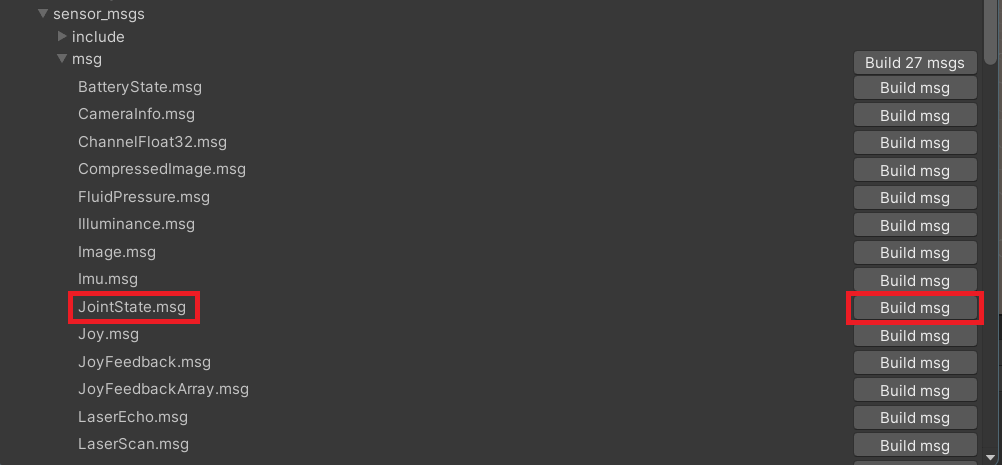
\includegraphics[width=0.75\linewidth]{figs/unityjoint_state_message.png}
        \caption{JointState message generation in Unity, corresponding to the desired ROS message}
        \label{fig:unityjoint_state_message}
        \end{figure}
        \item \textbf{Compiling and Verifying the Message Classes:} After generating the message classes, I compiled them in the Windows environment, ensuring they matched the expected structure as described in the UnityRoboticsTutorial repository. This process took some time to fully understand, but was critical for the successful integration of ROS data into Unity.
    \end{enumerate}



\section{Position Control (1 control type) - Unity to ROS} - confirm the purpose of this section - remove it?
    This control type enables operators to interact directly with the robot's joints in real-time, providing a responsive and highly interactive control environment. The implementation of Position Control involves several key steps to ensure seamless operation and integration with the ROS environment.
    
    \subsection{Saving and Sending Joint States}
    The first step in implementing Position Control was to capture and save the current states of the robot's joints in Unity. These joint states are then packaged and sent to the ROS environment upon user command. This process involves:
    \begin{enumerate}
        \item \textbf{Capturing Joint States:} The Unity application continuously monitors and records the positions of each joint of the digital twin robot, visible in the debug console represented in the figure \ref{fig:debug_joint_state}
        \begin{figure}[htpb]
            \centering
            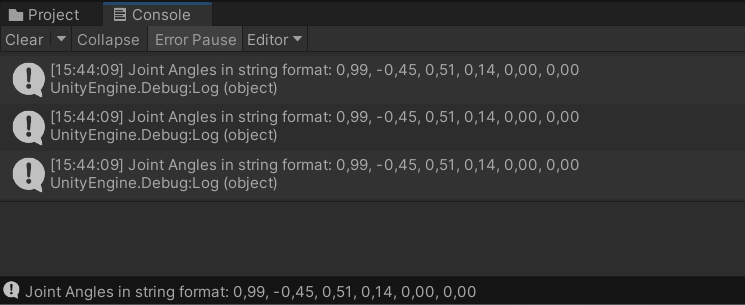
\includegraphics[width=0.8\linewidth]{figs/JointState_debug.png}
            \caption{Unity debug console showing the current digital twin's joint positions}
            \label{fig:debug_joint_state}
        \end{figure}
        \item \textbf{Data Serialization:} The joint states are serialized into a format suitable for transmission over the network. This was done by updating the joint positions into a list that is constantly saved into a JSON format, as depicted in the picture \ref{fig:json_pub}.
            \begin{figure}[htbp]
            \centering
            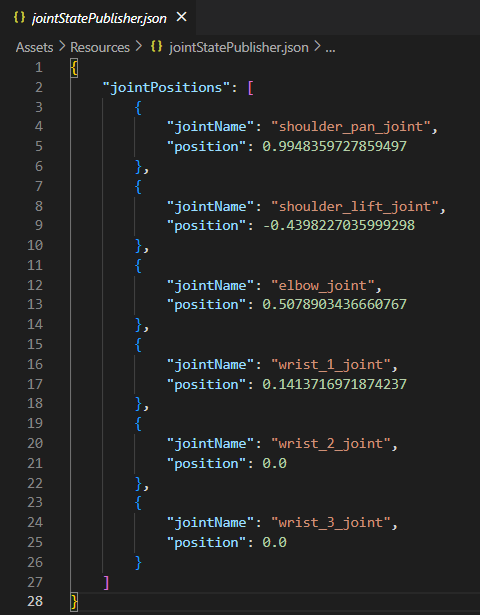
\includegraphics[width=0.5\linewidth]{figs/joint_states_json.png}
            \caption{JSON format used to store Unity's digital twin joint states}
            \label{fig:json_pub}
            \end{figure}
        \item \textbf{Sending Data:} Upon pressing a UI button trigger the serialized joint states are sent from Unity to the ROS environment using the previously established TCP/IP connection.
            %% versao com publish a cinzento - qual manter
            % \begin{figure}[htpb]
            %     \centering
            %     \includegraphics[width=0.8\linewidth]{figs/UI_Publish_button.png}
            %     \caption{UI Interface with Publishing button to send Unity's robot joint states into ROS the environment}
            %     \label{fig:publish_UI_button}
            % \end{figure}
    \end{enumerate}


    \subsection{ROS Integration for Position Control}
    In order to receive the data, the ROS environment needed some adjustments to process these joint states coming from Unity environment. Two new nodes were added to the ROS setup, enabling the following key functionalities:
    \begin{enumerate}
        \item \textbf{Joint State Listener Node:}
        \begin{itemize}
            \item \textbf{Purpose:} Receives joint states from Unity, ensuring that the digital inputs are translated into actionable data within the ROS environment.
            \item \textbf{Functionality:} This node listens to a dedicated topic from Unity, processes this data, and republishes it to a different control topic. Figure \ref{fig:json_sent_ros} illustrates an example of data transmitted from Unity to ROS. The accompanying debug log below demonstrates its accuracy.

            \begin{figure}
                \centering
                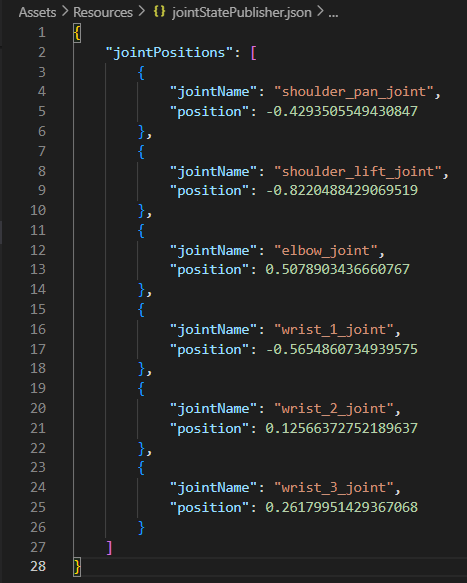
\includegraphics[width=0.5\linewidth]{figs/json_publisher_14h25.png}
                \caption{JSON file containing the unity's joint states that were sent to ROS environment}
                \label{fig:json_sent_ros}
            \end{figure}
            \begin{verbatim}
                    rosrun iris_ur10e unity_joint_subscriber.py 
                    [INFO] [1725629583.306162, 720.978000]: 
                    /joint_state_listener_7441_1725629572125I 
                    heard (-0.4293505549430847, -0.8220488429069519,
                    0.5078903436660767, -0.5654860734939575,
                    0.12566372752189636, 0.26179951429367065)
            \end{verbatim}
        \end{itemize}
            
        \item \textbf{Robot Control Node:}
            \begin{itemize}
                \item \textbf{Purpose:} Directly controls the robot's movements based on processed joint states from Unity.
                \item \textbf{Functionality:} This node requires that the previous one is also running, and subscribes to the control topic \textit{/move\_joint\_unity} to fetch and apply joint state data to the physical robot, mirroring the Unity operator’s interactions. The following debug log outputs the correct utilization of this node
                \begin{verbatim}
                    rosrun iris_sami move_unity.py 
                    [ INFO] [1725629576.546376282]: Loading robot model 'ur10e'...
                    [ INFO] [1725629577.773871662, 715.485000000]: Ready to take
                    commands for planning group manipulator.
                    [INFO] [1725629583.310087, 720.982000]: Moving arm to joint 
                    positions: (-0.4293505549430847, -0.8220488429069519,
                    0.5078903436660767, -0.5654860734939575,
                    0.12566372752189636, 0.26179951429367065)
                \end{verbatim}
            
                and the figure \ref{fig:synchronization-joint-control} displays two cases where the robot and its digital twin are properly synchronized using this control type.
            \end{itemize}
    \end{enumerate}
    
    \begin{figure}[b!]
        \centering
        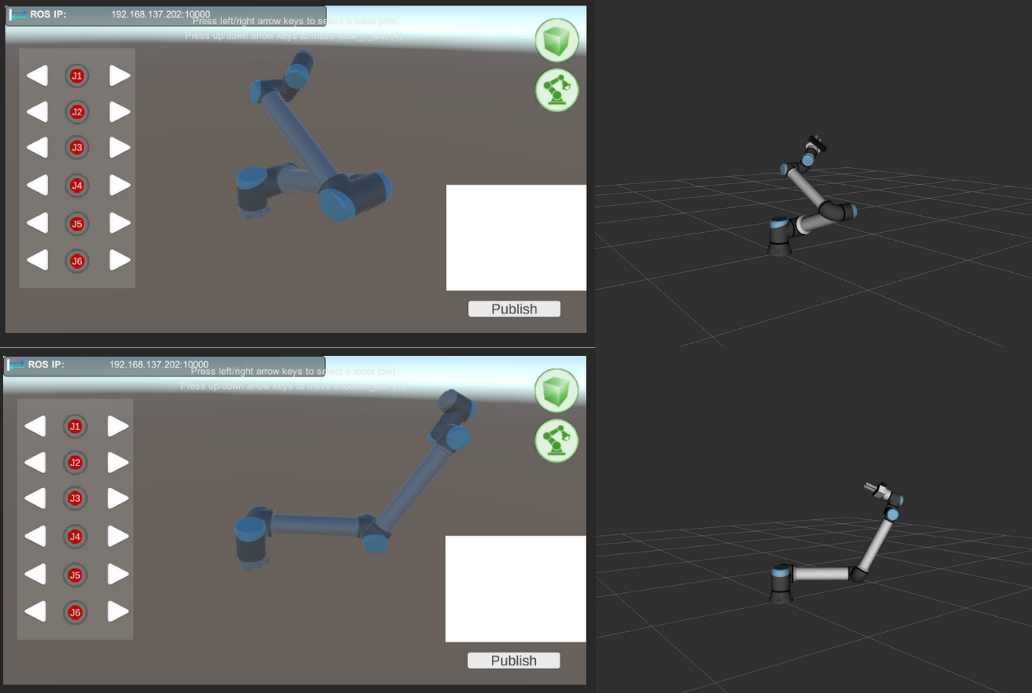
\includegraphics[width=1\linewidth]{figs/montagem.png}
        \caption{Two scenarios showcasing the synchronization between Unity and ROS environments using Joint Control}
        \label{fig:synchronization-joint-control}
    \end{figure}




    \section{Joint State Subscription (2 control type) - ROS to Unity}

    While the Position Control type allows operators to interactively manipulate the robot's joints and send these changes to the ROS environment, the Joint State Subscription control type operates in an opposite manner. It is designed to continually update the Unity digital twin's joint positions in synchronization with movements from the physical robot or its simulation in RViz. 


    \subsection{Saving ROS Data}
    In order to properly synchronize Unity's digital twin with real-time robot movements from the ROS environment, a new script \texttt{JointStateSubscriber.cs} was created. It subscribes to the \textit{/joint\_states} topic to continuously capture and store the robot's joint positions. This process is critical for maintaining a live reflection of the robot's state within the Unity simulation.
    
    \subsubsection{Subscribing to ROS Topics and Data Serialization}
    \begin{itemize}
        \item \textbf{Subscribing to Joint States:} The script actively listens to the \texttt{/joint\_states} topic, ensuring that any movement in the robot is promptly reflected in Unity.
        \item \textbf{Storing Joint Data:} Captured joint positions are stored in a C\# dictionary, facilitating efficient data access and manipulation.
        \item \textbf{Serializing Data to JSON:} The joint data is serialized into a JSON file, which provides a persistent and accessible format for storing the robot's state, overcoming potential restrictions from Unity packages that limit direct folder access.
    \end{itemize}
    
    \subsubsection{Explanation and Integration}
    The implementation of this system ensures that Unity's digital twin is consistently updated with the latest joint states from ROS, offering an accurate virtual representation for monitoring or interaction. Using the \texttt{SaveJointPositionsToFile()} method, joint data is structured and saved to enhance development workflow and project scalability.
    
    
    \subsubsection{Practical Application and Visualization}
    The real-time state of the robot’s joints, whether it is operating in a simulated environment or in real-time with the physical robot, is represented in figure \ref{fig:rviz_joint_states}.
    Initially, the script was designed to save these robot joints' values upon pressing a UI button, but it was later adapted to continuously update the \texttt{float64[] position} array from the ROS side, visible in the below terminal log snippet, into the Unity environment as shown in the figure \ref{fig:json_joint_states}, ensuring that the most recent joint positions were always available.
    
    
    \begin{figure}[h]
        \centering
        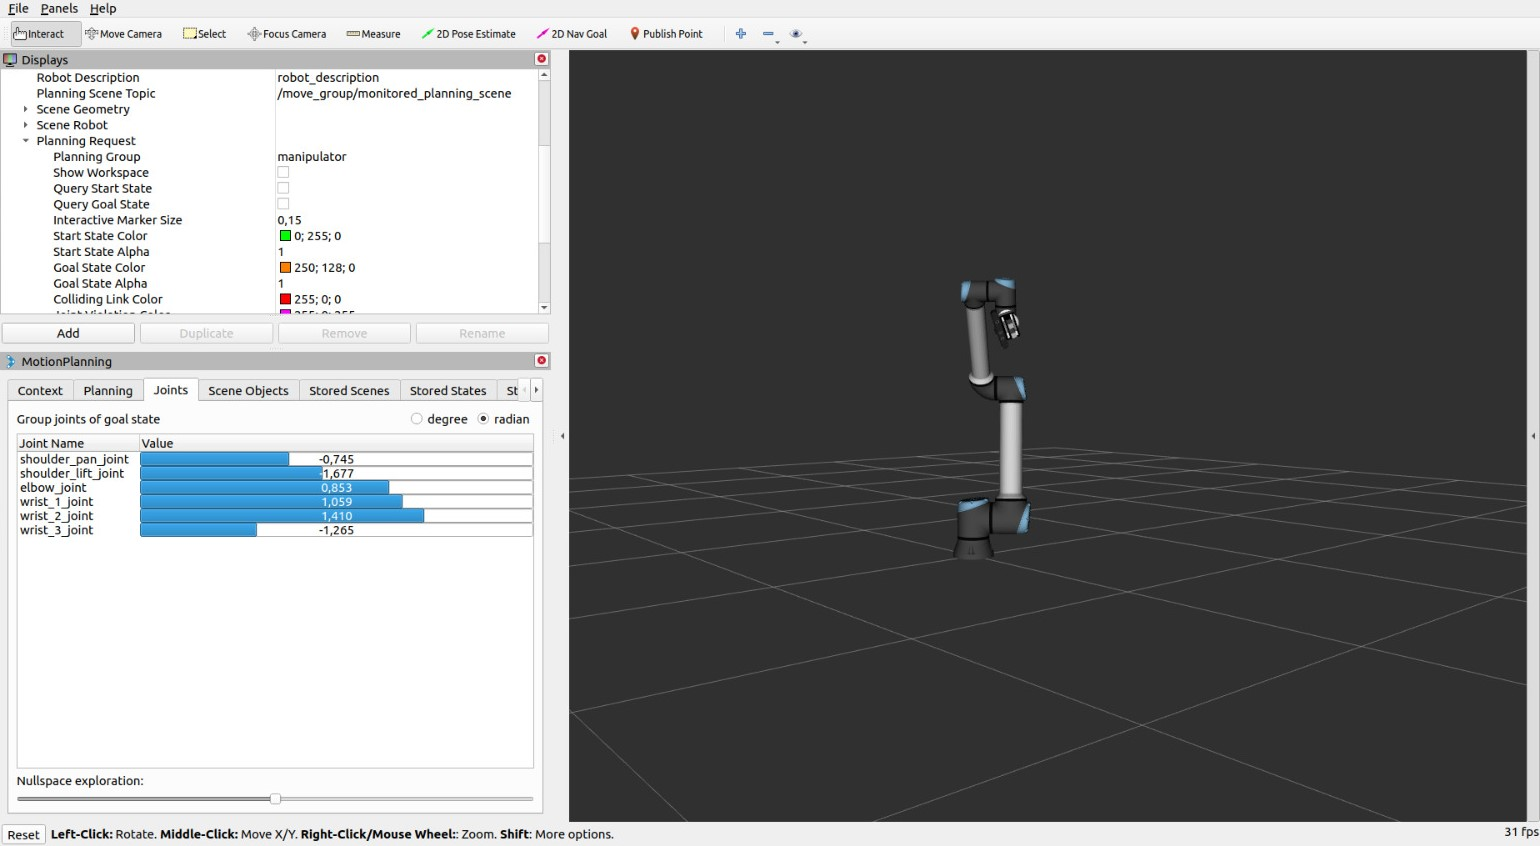
\includegraphics[width=\textwidth]{figs/jointStateSubRviz.png.jpg} % Adjust the file name and path as needed
        \caption{Rviz environment with simulated Robot and correspondent joint values, in radians}
        \label{fig:rviz_joint_states}
    \end{figure}
    
    
    \begin{verbatim}
    name:
        - elbow_joint
        - left_finger_joint
        - right_finger_joint
        - shoulder_lift_joint
        - shoulder_pan_joint
        - wrist_1_joint
        - wrist_2_joint
        - wrist_3_joint
    position: [0.8535921338670764, -5.695760001087214e-08, 5.587315793023694e-08, 
    -1.6766575764811593, -0.7445104810535929, 1.059219605892937, 1.410329834615414,
    -1.265097896821196]
    velocity: [-4.84869176906394e-05, -0.00020121543757810655, 0.0001987088475458378,
    0.006705746353461187, 0.00061522726960112, -0.0003380421322876756, 
    0.001088906936911304, 0.0002984877856849871]
    effort: [0.0, 0.0, 0.0, 0.0, 0.0, 0.0, 0.0, 0.0]
    \end{verbatim}
    
    \begin{figure}[h]
        \centering
        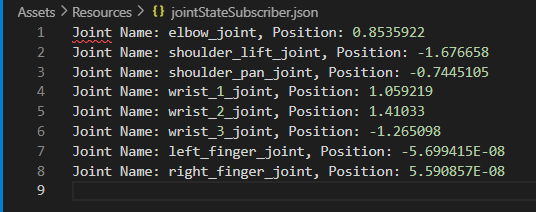
\includegraphics[width=0.8\textwidth]{figs/jsonJointStateSub.png}
        \caption{JointStateSubscriber Json file with Robot's joint values, in radians}
        \label{fig:json_joint_states}
    \end{figure}
    
    